\documentclass[10pt]{beamer}

\usepackage[utf8]{inputenc}
\usepackage[spanish, es-tabla]{babel}

\usetheme{metropolis}
\usepackage{appendixnumberbeamer}

\usepackage{booktabs}
\usepackage[scale=2]{ccicons}

\usepackage{pgfplots}
\usepgfplotslibrary{dateplot}

\usepackage{caption}
\usepackage{subcaption}

\usepackage{graphicx}

\usepackage{amsmath}
\usepackage{amsfonts}
\usepackage{amssymb}
\usepackage{amsthm}
\usepackage{esvect}

\usepackage{xspace}
\newcommand{\themename}{\textbf{\textsc{metropolis}}\xspace}

\title{Pump it Up. Equipo CharlaTED}
\author{Ignacio Aguilera Martos (<usuario>, KNN), Luis Balderas Ruiz (luisbalru, RIPPER), Francisco Luque Sánchez (<usuario>, <algoritmo>), Iván Sevillano García isega24, SVM}

\date{\today}
\institute{Preprocesamiento y Clasificación}

\begin{document}

\maketitle

\begin{frame}[fragile]{Contenidos}
\setbeamertemplate{section in toc}[sections numbered]
\tableofcontents[hideallsubsections]
\end{frame}

\section{SVM}
\begin{frame}
\frametitle{Preprocesamiento para SVM}

\begin{itemize}
	\item Eliminación de variables. 
	\begin{itemize}
		\item $region$, $recorded\_by$, $num\_private$,...
		\item Variables categóricas con más de 100 valores.
	\end{itemize}
	\pause
	\item Detección de valores perdidos(NA).
	\begin{itemize}
		\item $population = 0$??
		\item $construction\_year = 0$??
		\item Valores vacios.
	\end{itemize}
	\pause
	\item Cambiar tipos de dato.
	\begin{itemize}
		\item $region\_code$/$district\_code$ a factor.
		\item $date$ a numérico.
	\end{itemize}
\end{itemize}



\end{frame}


\begin{frame}

\frametitle{Limpieza de ruido e imputación de valores perdidos}

\begin{itemize}
	
	\item Limpieza de ruido mediante IPF\cite{ipf}.
	
	\item Amelia \cite{amelia} para valores perdidos numéricos(método iterativo de imputación).
	
	
	\item Imputación mediante KNN\cite{knnimputer} de valores categóricos(moda).
	
	
\end{itemize}

\end{frame}


\begin{frame}
\frametitle{PCA para variables dumificadas. Selección de subespacios relevantes. Selección de instancias.}

\begin{itemize}
	\item One hot encoding. Para cada valor las variables categórica, creamos una variable que valdrá 1 si la instancia tiene este valor.
	
	\item Normalizamos las variables.
	\item Aplicamos PCA\cite{pca} y nos quedamos con las variables cuya desviación típica sea mayor de un umbral(0.00001).
	\item Pasamos de 208 variables a 173.

	\item El método SMOTE\cite{smote} genera instancias de la clase minoritaria, sobrerepresentandola. 

\end{itemize}
\end{frame}

\begin{frame}
\frametitle{Flujo de información}
\begin{figure}
	\centering
	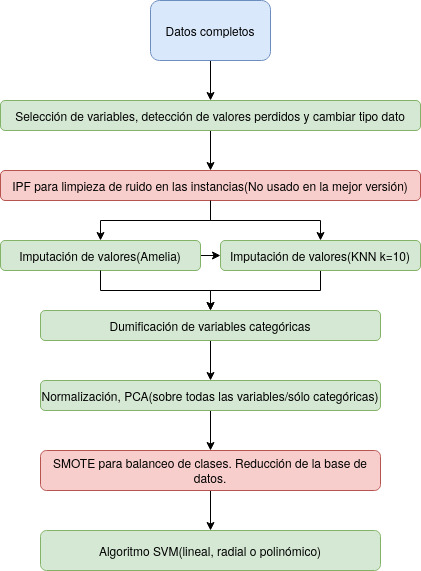
\includegraphics[width=0.5\linewidth]{figures/DiagramaFlujoSVM}
	\caption{Verde: Utilizado en el mejor modelo}
	\label{fig:diagramaflujosvm}
\end{figure}


\end{frame}


\begin{frame}
\frametitle{Puntuación a lo largo del tiempo de SVM}

\begin{figure}
	\centering
	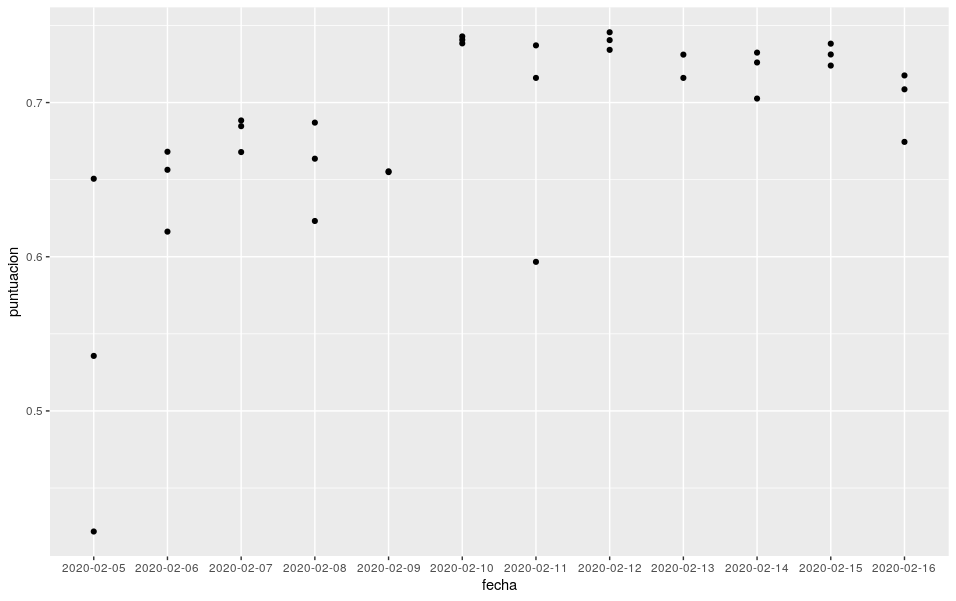
\includegraphics[width=\linewidth]{figures/puntuacionSVM}
	\caption{Máxima puntuación: 74.52\%,  12 de febrero}
	\label{fig:puntuacionsvm}
\end{figure}
Posición final: 2209


\end{frame}

\section{RIPPER}
\begin{frame}{Algoritmos y técnicas utilizados}
	\begin{itemize}
		\item \textbf{Ingeniería de características Selección y creación de características}
			\begin{itemize}
				\item Selección de variables semánticamente representativas. 
				\item LasVegas Wrapper. 
				\item Imputación de valores perdidos con media o mediana.
				\item Creación de características. \pause 
			\end{itemize}
		\item \textbf{Técnicas basadas en instancias. Selección, eliminación de ruido, sobremuestreo}
			\begin{itemize}
				\item ENN.
				\item IPF.
				\item SMOTE. Oversampling
				\item Random Undersampling. \pause 
			\end{itemize}
		\item \textbf{Ajuste de hiperparámetros.}
			\begin{itemize}
				\item Gridsearch de parámetros F (número de folds), N (mínimo peso de instancias) y O (número de ejecución para optimizar).
				\item 5-CV.
			\end{itemize}
	\end{itemize}
\end{frame}
\subsection{Técnicas que no dan resultados}
\begin{frame}{Problemas con LasVegasWrapper}
	contenidos...
\end{frame}

\subsection{Técnicas que dan resultados}



\section{KNN}
\begin{frame}{Pipeline empleado}
	\begin{figure}[H]
		\centering
		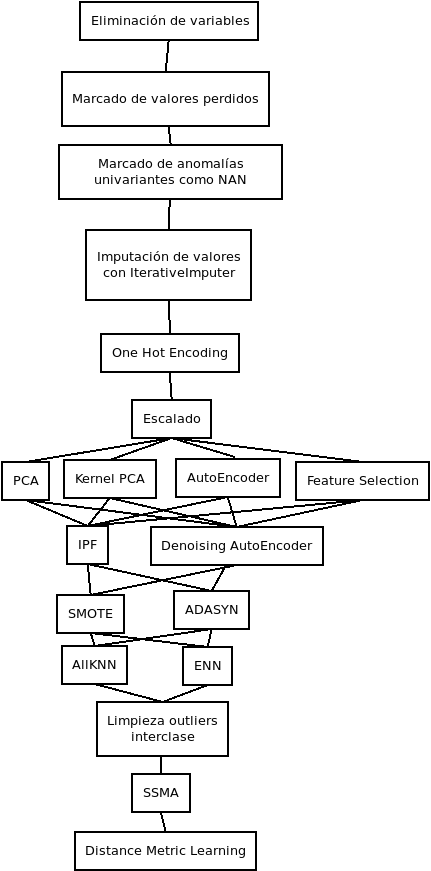
\includegraphics[scale=0.25]{./figures/knn/pipeline.png}
	\end{figure}
\end{frame}

\begin{frame}{Pipeline con mejor resultado}
	\begin{figure}[H]
		\centering
		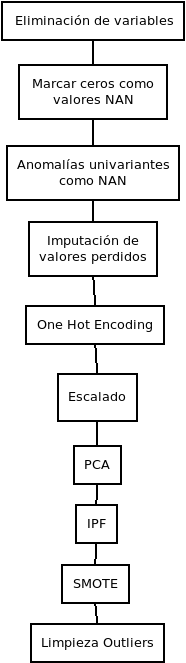
\includegraphics[scale=0.33]{./figures/knn/pipeline_final.png}
	\end{figure}
\end{frame}

\begin{frame}{Explicación de las técnicas}
	\vspace{10px}
	\pause
	\metroset{block=fill}
	\begin{block}{Eliminación de variables}
		Elimino las variables wpt\_name, subvillage, scheme\_name, funder, installer, ward, amount\_tsh y num\_private.
	\end{block}
	\pause
	\begin{block}{Marcado de anomalías como valores perdidos}
		En cada columna se calcula la media y la desviación típica. Aquellos datos que se salgan del intervalo $[media-5std, media+5std]$ se marcan como NAN.
	\end{block}
	\pause
	\begin{block}{Imputación iterativa}
		Empleamos una imputación iterativa sobre los valores perdidos.
	\end{block}
	\pause
	\begin{block}{PCA}
		Aplicamos PCA pero sólo sobre las columnas categóricas. El objetivo es explicar las variables categóricas mejor que en su codificación original. Reducimos a 44 variables todas las categóricas.
	\end{block}
\end{frame}

\begin{frame}{Explicación de las técnicas}
	\vspace{10px}
	\pause
	\metroset{block=fill}
	\begin{block}{IPF}
		Ejecutamos un IPF para limpiar el ruido con 4 iteraciones.
	\end{block}
	\pause
	\begin{block}{SMOTE}
		Hacemos un oversampling de las clases ''functional needs repair'' y ''non functional'' a 7500 y 22000 con respecto a 23500 de la clase ''functional'' con $k=7$.
	\end{block}
	\pause
	\begin{block}{Limpieza Outliers}
		Hacemos una limpieza de anomalías por cada clase eliminando el 1\% más anómalo según KNN con $k=7$ y la métrica de la mayor distancia.
	\end{block}
\end{frame}

\begin{frame}{Visualización de las técnicas}
	\begin{tabular}{ccc}
		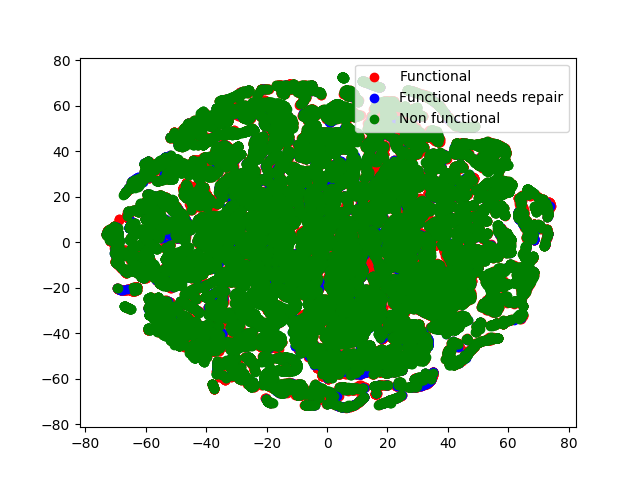
\includegraphics[scale=0.21]{./figures/knn/raw_2d.png} & 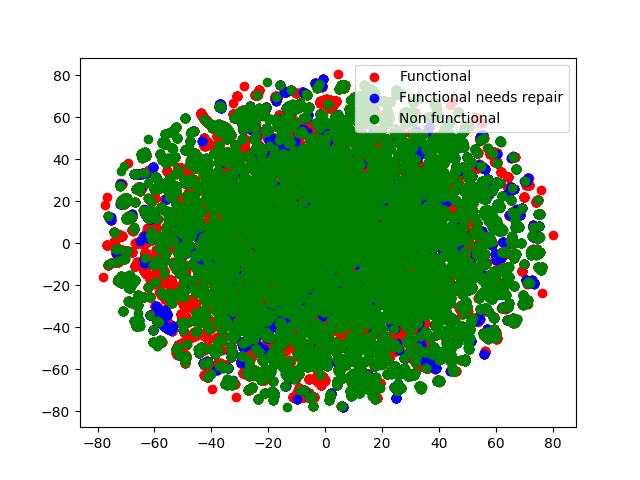
\includegraphics[scale=0.21]{./figures/knn/scaled_2d.png} & 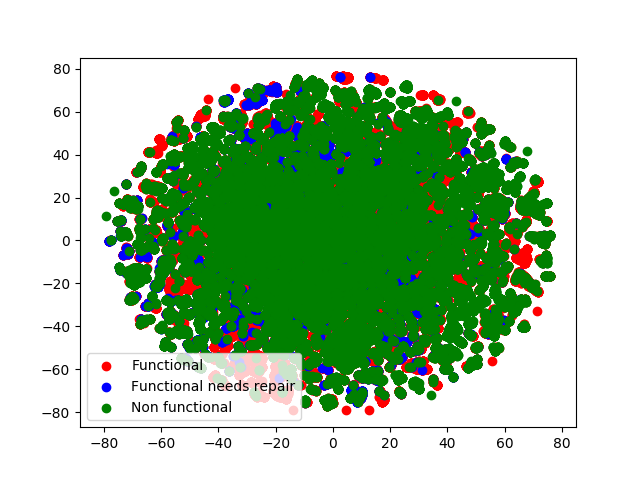
\includegraphics[scale=0.21]{./figures/knn/PCA_2d.png} \\
		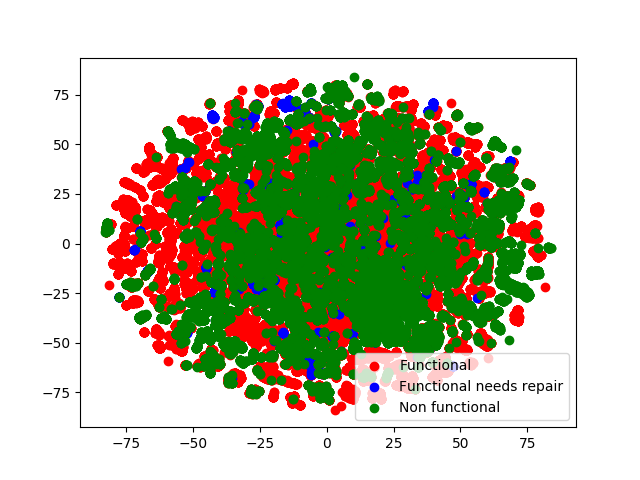
\includegraphics[scale=0.21]{./figures/knn/IPF_2d.png} & 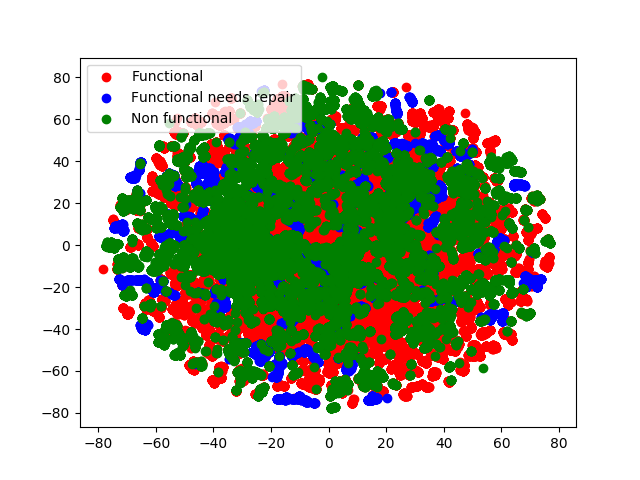
\includegraphics[scale=0.21]{./figures/knn/SMOTE_2d.png} & 
		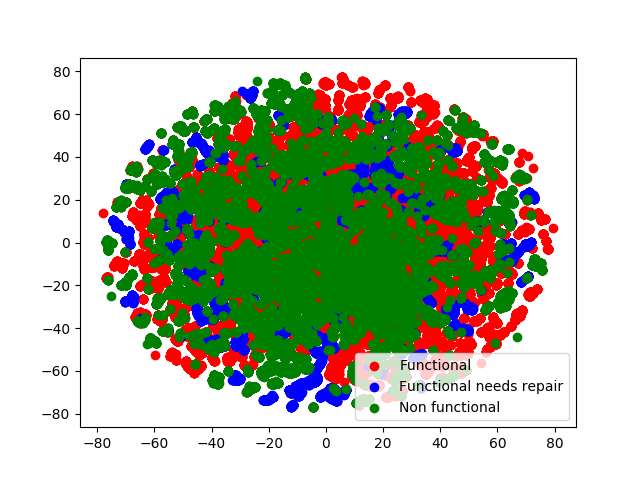
\includegraphics[scale=0.21]{./figures/knn/anomalias_knn_2d.png}
	\end{tabular}
\end{frame}

\begin{frame}{Posición en DrivenData}

	\begin{figure}[H]
		\centering
		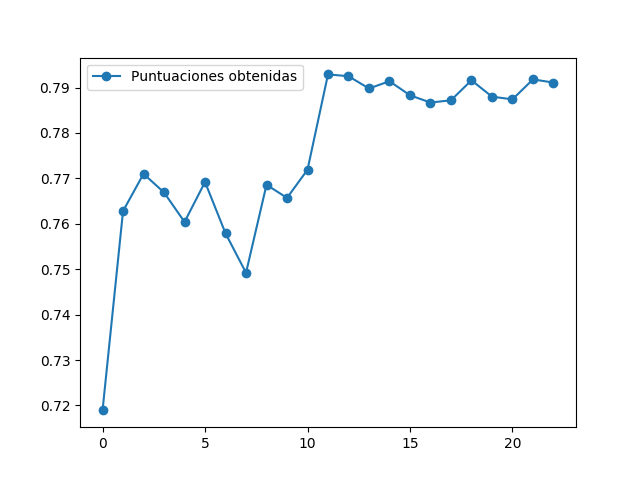
\includegraphics[scale=0.45]{./figures/knn/scores.png}
	\end{figure}

	\centering
	Puntuación final obtenida: 79.29\%
	
	Ranking final: 1729
	
	Número de subidas: 23
    
\end{frame}



\section{J48}
\begin{frame}{Primera aproximación}
  \metroset{block=fill}
  \begin{block}{Eliminación de variables}
    \begin{itemize}
    \item scheme\_name: 1/2 de valores perdidos
    \item Variables categóricas con más de 100 características
    \item recorded\_by: una única categoría
    \item region\_code: Correlada con district\_code
    \item construction\_year: Correlada con gps\_height y valores perdidos
      (valores 0 en esta columna no tienen sentido)
    \end{itemize}
  \end{block}
  \begin{block}{Imputación de valores perdidos}
    \begin{itemize}
    \item Variables numéricas: valor medio
    \item Variables categóricas: valor modal
    \end{itemize}
  \end{block}
  \begin{block}{Resultado}
    0.7677
  \end{block}
\end{frame}

\begin{frame}{Mejoras a dicha aproximación}
  \metroset{block=fill}
  \begin{block}{Eliminación de filas con missing values}
    \begin{itemize}
    \item Quedan 49841 filas en el conjunto
    \item Precisión: 0.7328 $\rightarrow$ se descarta la vía
    \end{itemize}
  \end{block}
  \begin{block}{Imputación en train por clase}
    \begin{itemize}
    \item En lugar de la media y la moda globales, se imputa por media
      y mediana de la clase
    \item En test, seguimos imputando igual
    \item Precisión: 0.7677 $\rightarrow$ no mejora el resultado, se
      descarta
    \end{itemize}
  \end{block}
  \begin{block}{Creación de una nueva categoría para los valores perdidos}
    \begin{itemize}
    \item En las variables categóricas se añade una categoría nueva,
      que representa el valor perdido.
    \item Precisión: 0.7385 $\rightarrow$ se descarta la vía
    \end{itemize}
  \end{block}
\end{frame}

\begin{frame}{Segundo estudio - importancia de las variables}
  \metroset{block=fill}
  \begin{block}{Medición de la importancia de las variables}
    Para las variables numéricas con valores perdidos en
    entrenamiento, se computa el valor de dichas variables con la
    media de los valores de la clase, dejando el resto de variables
    imputadas de forma poco inteligente.\\\\

    Tras esto, se clasifica el conjunto de entrenamiento con
    validación cruzada.
  \end{block}
  \begin{block}{Intuición}
    Las variables que produzcan una mejora importante en el resultado
    contendrán información relevante para la solución del problema.
  \end{block}
\end{frame}

\begin{frame}{Segundo estudio - importancia de las variables}
  \metroset{block=fill}
  \begin{block}{Resultados}
    Mejora escasa o nula en todas las variables.\\\\

    Imputación correcta de \texttt{construction\_year} $\rightarrow$
    Mejora en la CV de 0.78 a 0.84.\\\\

    La variable \texttt{construction\_year} parece muy relevante a
    la hora de establecer la clasificación
  \end{block}
\end{frame}


\begin{frame}[allowframebreaks]
\frametitle{Referencias}
\bibliographystyle{amsalpha}
\bibliography{referencias.bib}
\end{frame}

\begin{frame}[standout]
\LARGE{¿Preguntas?}
\vspace{10px}

\end{frame}


\end{document}